\documentclass[a4j,12pt,]{jarticle}
 \usepackage{float}
 \usepackage{siunitx} %%SI単位系用
 \usepackage{amssymb, amsmath}
 \usepackage{ascmac,here,txfonts}
 \usepackage{hyperref}
 \usepackage{listings}
 \usepackage{pxjahyper}
 \usepackage[dvipdfmx]{graphicx}
 \usepackage{amssymb, amsmath}
  \usepackage{listings}
  \usepackage[dvipdfmx]{color}

  \lstset{
    language={Python},
    basicstyle={\ttfamily},
    identifierstyle={\small},
    commentstyle={\small\itshape},
    keywordstyle={\small\bfseries},
    ndkeywordstyle={\small},
    stringstyle={\small\ttfamily},
    frame={single},
    breaklines=true,
    columns=[l]{fullflexible},
    numbers=left,
    xrightmargin=0zw,
    xleftmargin=3zw,
    numberstyle={\scriptsize},
    stepnumber=1,
    numbersep=1zw,
    lineskip=-0.5ex,
  }

\begin{document}

{\noindent\small 第21回報告書 \hfill\today}
\begin{center}
  {\Large Elasticsearchのバージョンアップ}
\end{center}
\begin{flushright}
  祖父江匠真 \\
\end{flushright}

\section{概要}
リサイクル館の太陽光パネルの計測データを保存しているElasticsearchシステム(133.71.201.197)はバージョン7.17.6であり, CO\textsubscript{2}データを保存しているElasticsearchシステム(133.71.106.141, 133.71.106.170, 133.71.106.136)はバージョン7.17.9である.

これらの異なるバージョンのElasticsearchノードでクラスタを構築することは出来ないため, Elasticsearchをバージョンアップする必要がある. そこで今回は, 133.71.201.197にインストールされたElasticsearchのバージョンアップ作業について報告する.

\section{バージョンアップ手順}

\subsection{インストール方法の特定}

バージョンアップを行うためには, 133.71.201.197のUbuntuPCにどのようにElasticsearchをインストールしたか特定する必要がある.

図 \ref{p1}に, aptによってインストールされたパッケージの中にelasticsearchという文字列を含むパッケージが存在するか調べた結果を示す.
図 \ref{p1}より, aptによってインストールされたことが分かった.

\begin{figure}[H]
  \begin{center}
    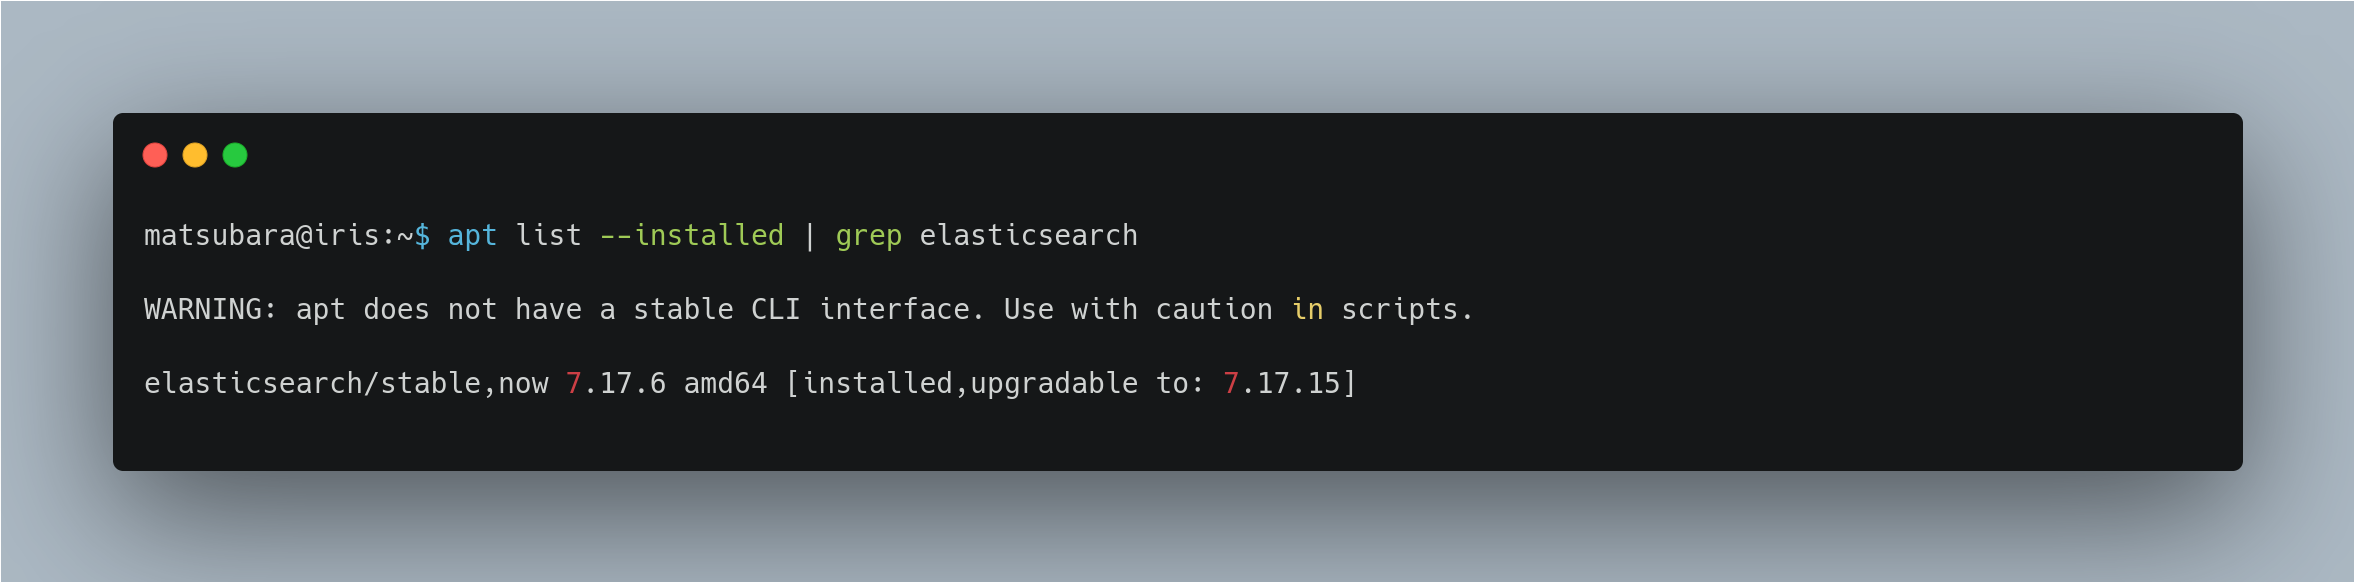
\includegraphics[width=160mm]{apt-grep.png}
    \caption{aptによってelasticsearchがインストールされたか調べた結果}
    \label{p1}
  \end{center}
\end{figure}

次に, aptでインストール可能なelasticsearchのバージョンを一覧表示した結果を図 \ref{p2}に示す. 図 \ref{p2}にターゲットである7.17.9が含まれているため, aptを使用してバージョンアップできることが確認できた.

\begin{figure}[H]
  \begin{center}
    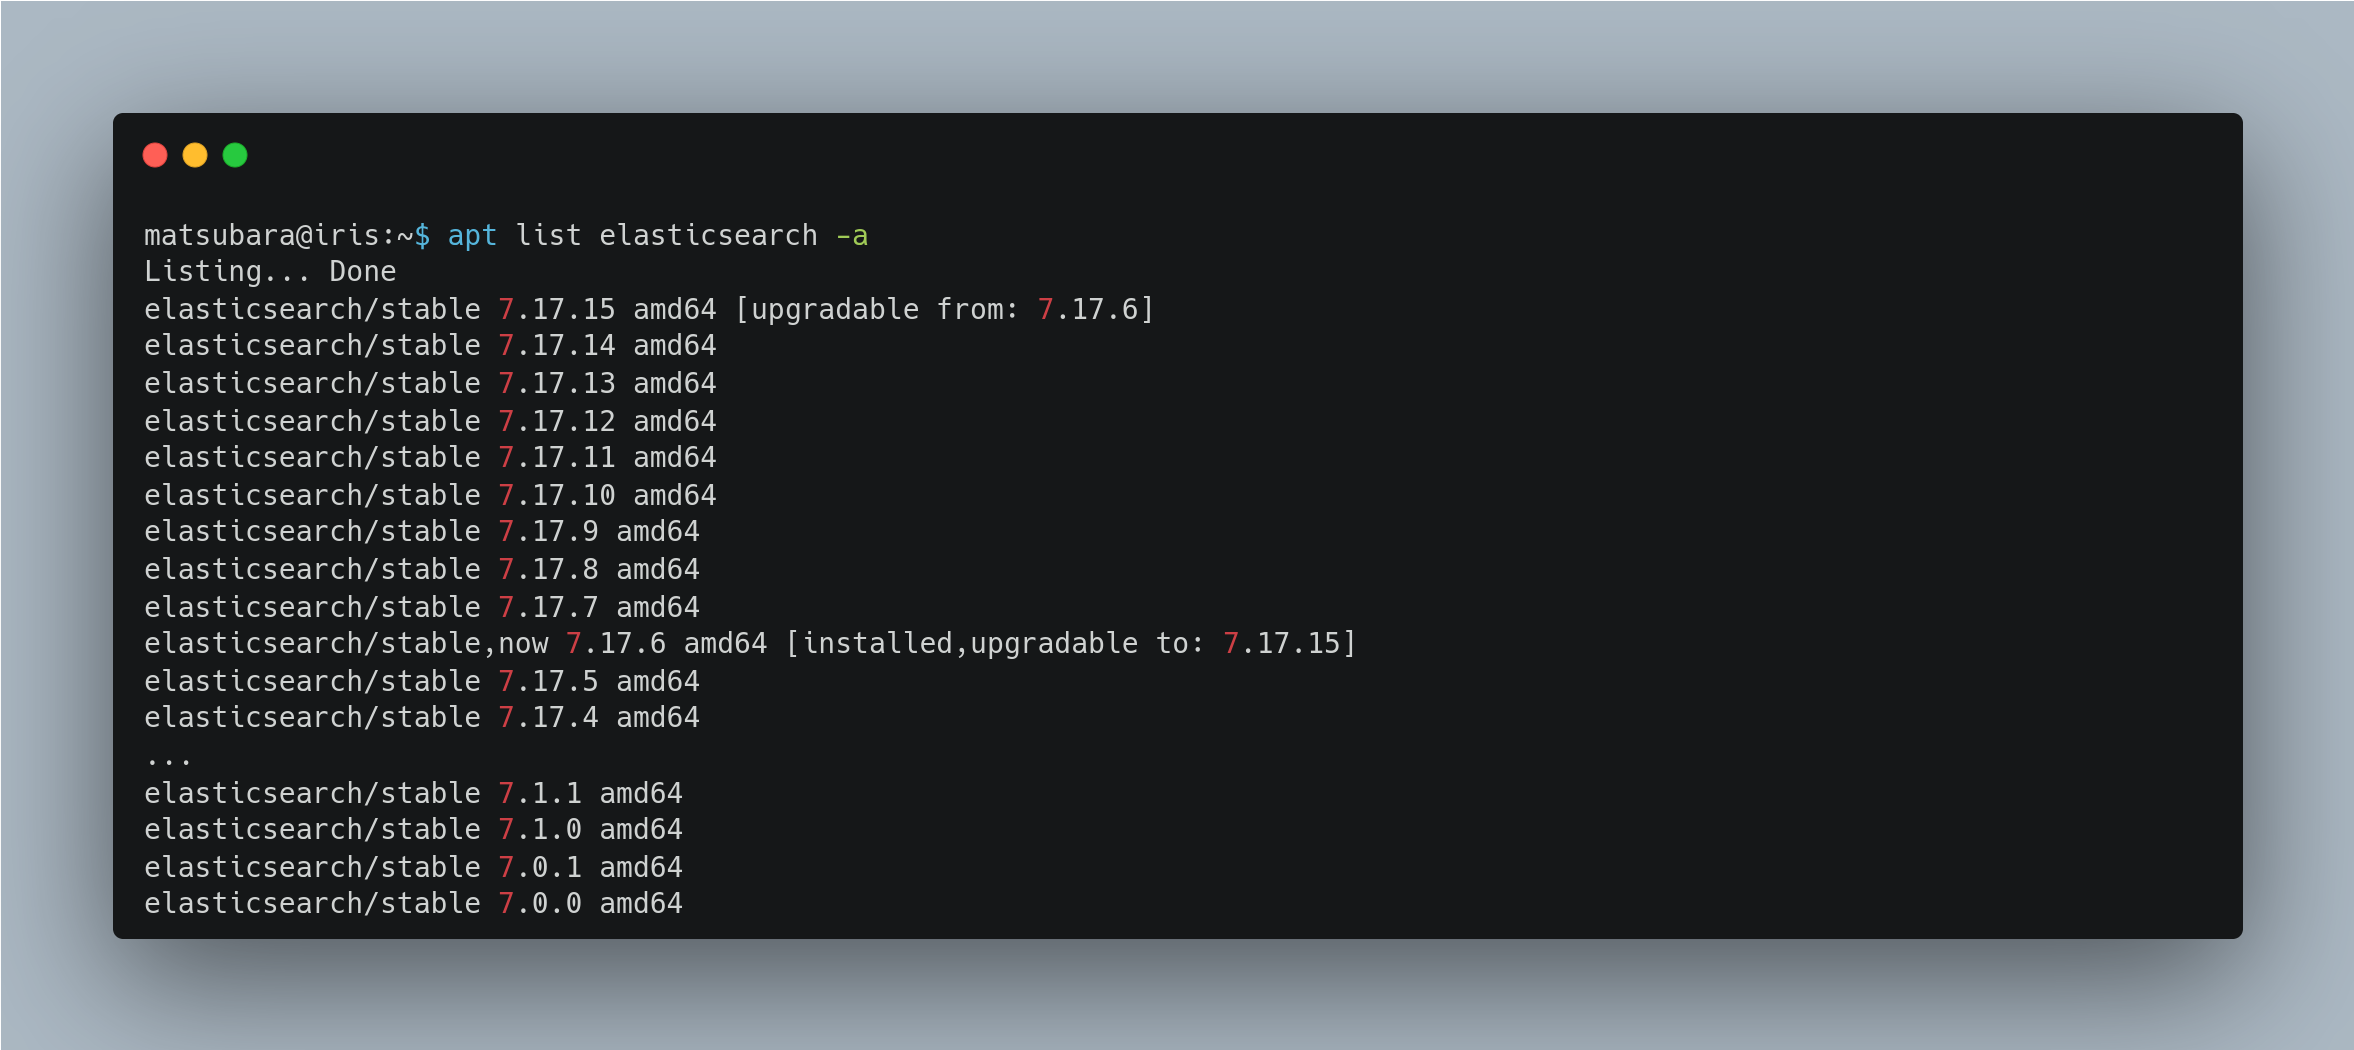
\includegraphics[width=160mm]{apt-list.png}
    \caption{aptでインストール可能なelasticsearchのバージョンを一覧表示した結果}
    \label{p2}
  \end{center}
\end{figure}

\subsection{aptによるバージョンアップ}

まず, \textbf{sudo systemctl stop elasticsearch.service}コマンドを実行してelasticsearchノードをシャットダウンする.

次に, \textbf{sudo apt install elasticsearch=7.17.9}コマンドを実行してelasticsearchパッケージをバージョンアップする.

elasticsearchをバージョンアップ後, \textbf{sudo systemctl start elasticsearch}コマンドを実行してelasticsearchノードを起動する.

ノードの起動後, elasticsearchのバージョンを確認した結果を図 \ref{p3}に示す.

\begin{figure}[H]
  \begin{center}
    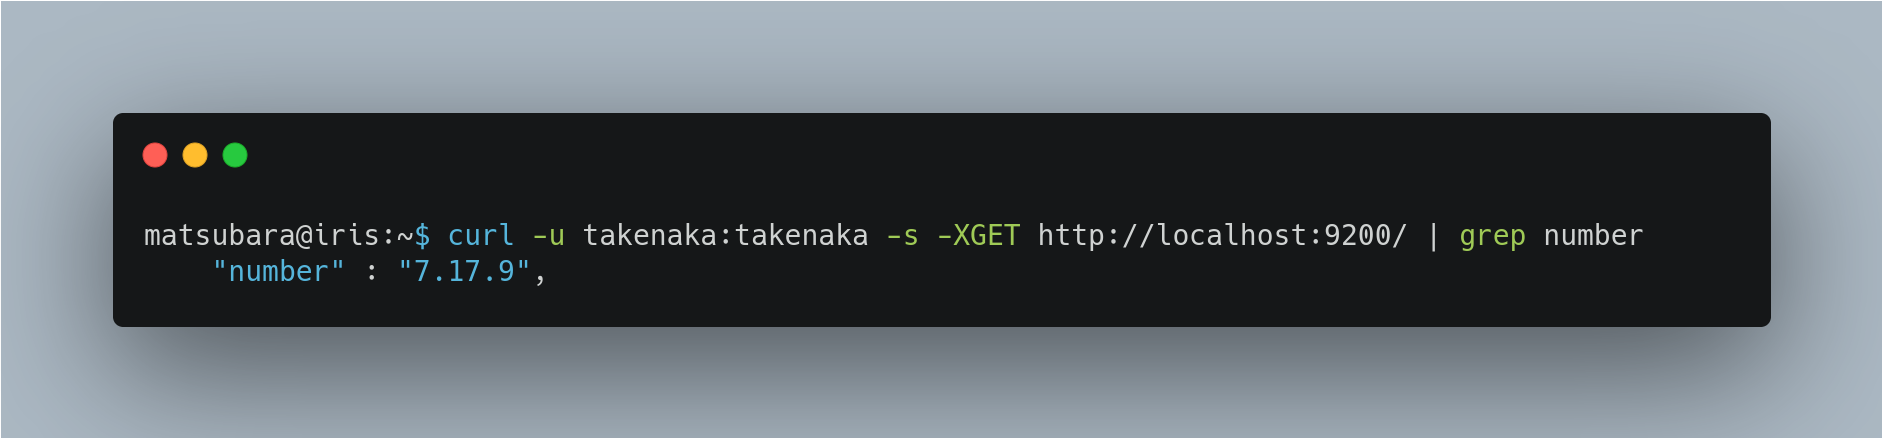
\includegraphics[width=160mm]{version-check.png}
    \caption{ノードの起動後, elasticsearchのバージョンを確認した結果}
    \label{p3}
  \end{center}
\end{figure}

図 \ref{p3}より, Elasticsearchのバージョンが7.17.9にバージョンアップ出来たことが確認できた.

\section{kibanaのバージョンアップ}

kibanaもelasticsearchと同様, aptを使用してインストールされていたため, \textbf{sudo systemctl stop kibana.service}コマンド, \textbf{sudo apt install kibana=7.17.9}, \textbf{sudo systemctl start elasticsearch}コマンドをそれぞれ実行して, kibanaのバージョンアップを行った.

\section{バージョンアップ後の動作確認}

elasticsearchのバージョンアップ後, 太陽光パネルの計測データがElasticsearchに保存されているかkibana上で確認した結果を図 \ref{p4}に示す.

\begin{figure}[H]
  \begin{center}
    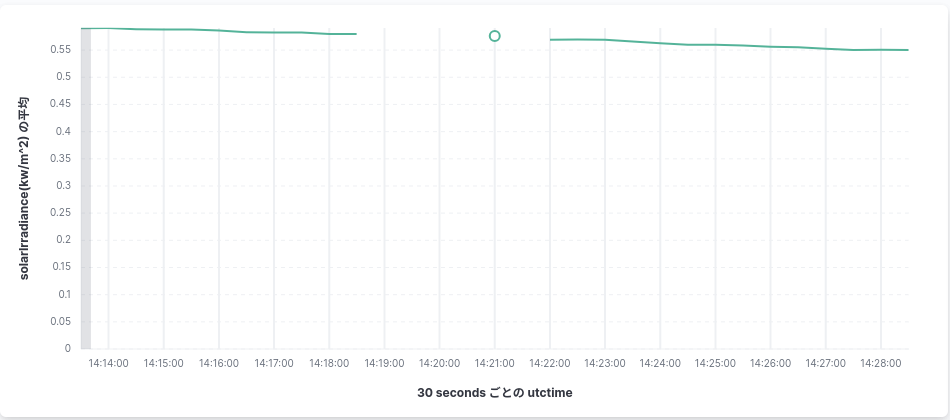
\includegraphics[width=160mm]{downtime.png}
    \caption{Elasticsearchのバージョンアップ後, 太陽光パネルの計測データが保存されているかkibana上で確認した結果}
    \label{p4}
  \end{center}
\end{figure}

図 \ref{p4}より, バージョンアップ後のElasicsearchノードを起動した14:22:00以降にドキュメントがインサートされていることが確認できた.

\section{まとめ}
今回は, 133.71.201.197にインストールされたElasticsearchのバージョンアップ作業について報告した.

次回は, インデックスが既に存在するElasticsearchノードを使用してクラスタを構築した際に, 既存インデックスのデータを失うことなくクラスタを構築できるか検証した結果について報告する.

\begin{thebibliography}{5}
  \bibitem{1}Elasticsearch B.V.,\\ ”https://www.elastic.co/guide/en/elasticsearch/reference/7.17/rolling-upgrades.html”, https://www.elastic.co/guide/en/elasticsearch/reference/7.17/rolling-upgrades.html, 参照 Dec 4,2023.
\end{thebibliography}

\end{document}

